\label{chapter:fif}
%\begin{itemize}
%	\item Bias -> fairness metric 
%	\item Fairness influence function (FIF)
%	\item Example
%	\item Contribution (1) framework (2) algorithm (3) experimental validation
%	\item Related works.
%	\item Notation paragraph
%\end{itemize}

%The past few decades have witnessed a remarkable advancement in the field of machine learning, with its applications encompassing crucial decision-making processes such as college admissions~\cite{martinez2021using}, recidivism prediction~\cite{tollenaar2013method}, job applications~\cite{ajunwa2016hiring}, and more.  In such applications, the deployed machine learning classifier often demonstrates bias towards certain demographic groups present in the data~\cite{dwork2012fairness}. For instance, a machine learning classifier employed in college admissions may show a disproportionate preference for White-male candidates over Black-female candidates. This can occur due to historical biases present in the admission data, the classifier's accuracy-focused learning objective, or a combination of the two~\cite{landy1978correlates,zliobaite2015relation,berk2019accuracy}. Following such phenomena, multiple group-based fairness metrics, such as \textit{statistical parity}, \textit{equalized odds}, \textit{predictive parity}, etc.\ have been proposed to quantify the bias of the classifier on a dataset.  For example, a statistical parity of $ 0.6 $ for the college admission classifier would indicate that White-male candidates are offered admission $ 60\% $ more frequently than Black-female candidates~\cite{garg2020fairness,besse2021survey}.


In this chapter, we envision towards combining two research themes in the thesis: interpretability and fairness, and discuss an algorithmic framework to interpret or explain fairness in machine learning.
As demonstrated in Chapter~\ref{chapter:justicia} and~\ref{chapter:fvgm}, fairness metrics measure global bias, but do not detect or explain its sources~\cite{begley2020explainability,lundberg2020explaining,pan2021explaining}.
In order to diagnose the emergence of bias in the predictions of classifier, it is important to compute explanations, such as how different features attribute to the global bias. Motivated by the GDPR's ``right to explanation'', research on explaining model predictions~\cite{ribeiro2016should,lundberg2017unified,lundberg2020local2global} has surged, but explaining prediction bias has received less attention~\cite{begley2020explainability,lundberg2020explaining}. In order to identify and explain the sources of bias and also the impact of affirmative/punitive actions to alleviate/deteriorate bias, it is important to understand \textit{which features contribute how much to the bias of a classifier} applied on a dataset. To this end, we follow a global feature-attribution approach to explain the sources of bias, where we relate the \emph{influences} of input features towards the resulting bias of the classifier. In this context, existing bias attributing methods~\cite{begley2020explainability,lundberg2020explaining} are variants of local function approximation~\cite{sliwinski2019axiomatic}, whereas bias is a global statistical property of a classifier. Thus, \textit{we aim to design a bias attribution method that is global by construction}. In addition, existing methods only attribute the individual influence of features on bias while neglecting the \textit{intersectionality} among features. Quantifying intersectionality allows us to explain bias induced by the higher-order interactions among features; hence accounting for intersectionality is important to understand bias as suggested by recent literature~\cite{buolamwini2018gender,wang2022towards}. 
%\textit{By attributing bias to both individual and intersecting features, we can gain a more detailed understanding of bias} and pave the way for designing more effective fairness algorithms. 
In this chapter, \textit{we aim to design a global bias attribution framework and a corresponding algorithm that can quantify both the individual and intersectional influences of features leading to granular and functional explanation of the sources of bias.}


\paragraph{Contributions.}  Our contributions are three-fold.

\begin{enumerate}
	
	\item \textbf{Formalism:} We propose to measure the contribution of individual and intersectional features towards the bias of a classifier operating on a dataset by estimating their \textbf{F}airness \textbf{I}nfluence \textbf{F}unctions (FIFs) (Section~\ref{fairness_fairXplainer_sec:fifs}). Our method is based on transforming existing fairness metrics into the difference of scaled conditional variances of classifier's prediction, which we then decompose using Global Sensitivity Analysis (GSA)\textemdash a standard technique recommended by regulators to assess numerical models\cite{eu,usepa}. FIFs have several desirable properties (Theorem~\ref{fairness_fairXplainer_thm:fif_property}), including the decomposability property~\cite{begley2020explainability,lundberg2020explaining}. This property states that the sum of FIFs of all individual and intersectional features equals the bias of the classifier. With this formulation of FIFs, we can identify which features have the greatest influence on bias by looking at the disparity in their scaled decomposed variance between sensitive groups.
	
%	\item \textbf{Formalism:} Given a classifier, a dataset, and a group fairness metric, we propose to estimate individual and intersectional \textbf{F}airness \textbf{I}nfluence \textbf{F}unctions (FIFs) of features as a measure of contribution towards the bias of the classifier induced by the features (Section~\ref{fairness_fairXplainer_sec:fifs}).	Our FIF formulation is based on representing existing fairness metrics as the difference of the scaled conditional variances of classifier's prediction, followed by a decomposition of variance according to Global Sensitivity Analysis (GSA)\textemdash a standard technique recommended by regulators to assess numerical models\cite{eu,usepa}. The presented FIF formulation results in different desired properties (Theorem~\ref{fairness_fairXplainer_thm:fif_property}): the efficiency property~\cite{begley2020explainability,lundberg2020explaining} states that the sum of FIFs of all subsets of features is equal to the bias of the classifier.  This allows us to view FIFs as a way to decompose the bias of the classifier among features. In this decomposition, features that demonstrate a higher disparity in the scaled decomposed variance of prediction between sensitive groups are attributed to be highly influential on the bias in prediction. 
	
	\item \textbf{Algorithmic:} We propose a new algorithm, called {\fairXplainer}, to estimate individual and intersectional FIFs of features given a dataset, a classifier, and a fairness metric. The algorithm is capable of working with any linear group fairness metric, including statistical parity, equalized odds, or predictive parity (Section~\ref{fairness_fairXplainer_sec:fairxplainer}). Building on GSA\cite{saltelli2008global} techniques, {\fairXplainer} solves a local regression problem~\cite{loader2006local} based on cubic splines~\cite{li2010global} to decompose the variance of the classifier's prediction among all the subsets of features.
	
%	\item \textbf{Algorithmic:} We instantiate an algorithm, {\fairXplainer}, for estimating FIFs of  features for a given classifier, a dataset, and any group fairness metric, namely statistical parity, equalized odds, or predictive parity (Section~\ref{fairness_fairXplainer_sec:fairxplainer}).  The key idea is to import techniques from GSA\cite{saltelli2008global} to decompose the variance of the classifier's prediction among all  subsets of features by applying a local regression technique~\cite{loader2006local} based on cubic splines~\cite{li2010global}. 
	
	\item \textbf{Experimental:} We evaluate  {\fairXplainer}  on a variety of real-world datasets and machine learning classifiers to demonstrate its efficiency in estimating the individual and intersectional FIFs of features. Our results show that {\fairXplainer} has a higher accuracy in approximating bias using estimated FIFs compared to existing methods (Section~\ref{fairness_fairXplainer_sec:experiments}). Our estimation of FIFs also shows a strong correlation with fairness interventions. Furthermore, {\fairXplainer} yields more granular explanation of the sources of bias by combining both individual and intersectional FIFs, and also detects patterns that existing fairness explainers cannot. Finally, {\fairXplainer} enables us to observe changes in FIFs as a result of different fairness enhancing algorithms~\cite{calmon2017optimized,hardt2016equality,kamiran2012decision,zemel2013learning,zhang2018mitigating,zhang2018fairness,zhang2019faht} and fairness reducing attacks~\cite{hua2021human,mehrabi2020exacerbating,solans2020poisoning}. This creates opportunities to further examine the impact of these algorithms.	
\end{enumerate}




\begin{figure}
	\begin{minipage}[t]{0.13\textwidth}			
		\scalebox{1}{	
		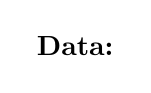
\begin{tikzpicture}[x=1cm,y=0.3cm]
		\node[] (a1) {\textbf{Data:}};			
		\end{tikzpicture}
		}
	\end{minipage}%
	\begin{minipage}{0.35\textwidth}
		\centering
		\subfloat[Dependency among features and prediction]{
			\scalebox{0.4}{	
				\begin{tikzpicture}[x=1.5cm,y=0.3cm]
				% Define nodes
				\node[latent,scale=2] (a1) {$\textrm{age}$} ; %
				\node[obs, scale=2, below=of a1, xshift=-2cm] (h) {$\textrm{fitness}$}; %
				\node[obs, scale=2, below=of a1, xshift=2cm] (i) {$\textrm{income}$}; %
				\node[obs, scale=2, below=of h, xshift=2cm] (p) {$\widehat{Y}$}; %			
				%%add edge
				\edge[] {a1} {h,i} ;
				\edge[] {h,i} {p} ;
				\end{tikzpicture}
			}	
			\label{fairness_fairXplainer_fig:dag_age_income_fitness}}
	\end{minipage}%
	\begin{minipage}{0.4\textwidth}
		\centering
		\subfloat[Age-dependent distributions of non-sensitive features]{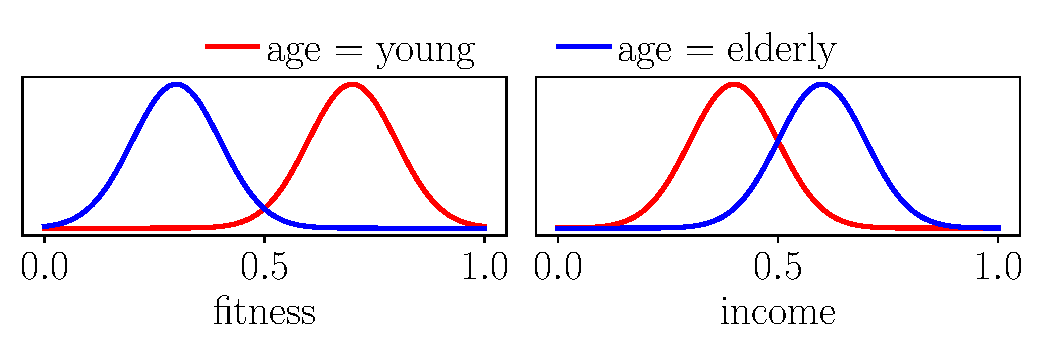
\includegraphics[scale=0.4]{figures/fairness/fif/sanity_distribution}
		\label{fairness_fairXplainer_fig:distribution_example}}
	\end{minipage}

	\begin{minipage}[t]{0.13\textwidth}
		\scalebox{1}{	
			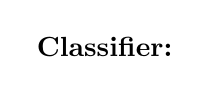
\begin{tikzpicture}[x=1cm,y=0.3cm]
			\node[] (a1) {\textbf{Classifier:}};			
			\end{tikzpicture}
		}
	\end{minipage}%
	\begin{minipage}{0.43\textwidth}
		\centering
		\subfloat[Decision tree (DT$ 1 $)]{
			\scalebox{0.45}{	
				\begin{tikzpicture}[x=1cm,y=1.8cm]
				\node [box, scale=1.5]                                    (p)      {fitness $\geq 0.61$};
				\node [scale=1.5, box, below= of p, xshift=-2.1cm, yshift=1.2cm]    (a1)    {income\\ $\geq 0.29$};
				\node [scale=1.5, box, below= of p, xshift=2.1cm, yshift=1.2cm]     (a2)    {income $\geq 0.69$};
				\node [scale=1.5,below= of a1, xshift=-1.5cm, yshift=0.8cm]  (a11)    { $\widehat{Y}= 1$};
				\node [scale=1.5,below= of a1, xshift=1.5cm, yshift=0.8cm]   (a12)    { $\widehat{Y}=0 $};
				\node [scale=1.5,below= of a2, xshift=-1.5cm, yshift=0.8cm]  (a21)    { $\widehat{Y}= 1$};
				\node [scale=1.5,below= of a2, xshift=1.5cm, yshift=0.8cm]  (a22)    { $\widehat{Y}= 0$};
				%
				\path [line] (p) -|         (a1) node [scale=1.5,midway, above]  {Y};
				\path [line] (p) -|         (a2) node [scale=1.5,midway, above]  {N};
				\path [line] (a1) -|       (a11) node [scale=1.5,midway, above]  {Y};
				\path [line] (a1) -|       (a12) node [scale=1.5,midway, above]  {N};
				\path [line] (a2) -|       (a21) node [scale=1.5,midway, above]  {Y};
				\path [line] (a2) -|       (a22) node [scale=1.5,midway, above]  {N};
				\end{tikzpicture}}
			\label{fairness_fairXplainer_fig:dt_original}}
	\end{minipage}%
	\begin{minipage}{0.45\textwidth}
		\centering
		\subfloat[Decision tree with an affirmative action (DT$ 2 $)]{
			\scalebox{0.45}{	
				\begin{tikzpicture}[x=1cm,y=1.8cm]
				\node [box, scale=1.5]                                    (p)      {fitness $\geq 0.61$};
				\node [scale=1.5, box, below= of p, xshift=-2.1cm, yshift=1.2cm]    (a1)    {income\\ $\geq 0.29$};
				\node [scale=1.5, box, below= of p, xshift=2.1cm, yshift=1.2cm, fill=affirmative]     (a2)    {income $\geq 0.55$};
				\node [scale=1.5,below= of a1, xshift=-1.5cm, yshift=0.8cm]  (a11)    { $\widehat{Y}= 1$};
				\node [scale=1.5,below= of a1, xshift=1.5cm, yshift=0.8cm]   (a12)    { $\widehat{Y}=0 $};
				\node [scale=1.5,below= of a2, xshift=-1.5cm, yshift=0.8cm]  (a21)    { $\widehat{Y}= 1$};
				\node [scale=1.5,below= of a2, xshift=1.5cm, yshift=0.8cm]  (a22)    { $\widehat{Y}= 0$};
				%
				\path [line] (p) -|         (a1) node [scale=1.5,midway, above]  {Y};
				\path [line] (p) -|         (a2) node [scale=1.5,midway, above]  {N};
				\path [line] (a1) -|       (a11) node [scale=1.5,midway, above]  {Y};
				\path [line] (a1) -|       (a12) node [scale=1.5,midway, above]  {N};
				\path [line] (a2) -|       (a21) node [scale=1.5,midway, above]  {Y};
				\path [line] (a2) -|       (a22) node [scale=1.5,midway, above]  {N};
				\end{tikzpicture}}	
			
			\label{fairness_fairXplainer_fig:dt_affirmative}}
	\end{minipage}

	\begin{minipage}[t]{0.07\textwidth}
		%\vspace{-2em}
		\scalebox{1}{	
			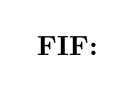
\begin{tikzpicture}[x=1cm,y=0.3cm]
			\node[] (a1) {\textbf{FIF:}};			
			\end{tikzpicture}
		}
	\end{minipage}%
	\begin{minipage}{0.46\textwidth}
		\centering
		\subfloat[Fairness influence functions (FIF) for DT$ 1 $]{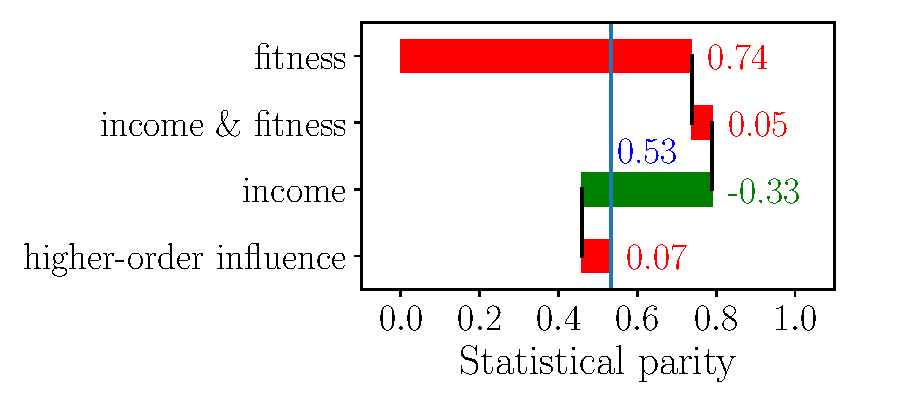
\includegraphics[scale=0.42]{figures/fairness/fif/fif_example}
		\label{fairness_fairXplainer_fig:fif_original}}	
	\end{minipage}%
	\begin{minipage}{0.5\textwidth}
		\centering
		\subfloat[Modified FIFs for DT$ 2 $]{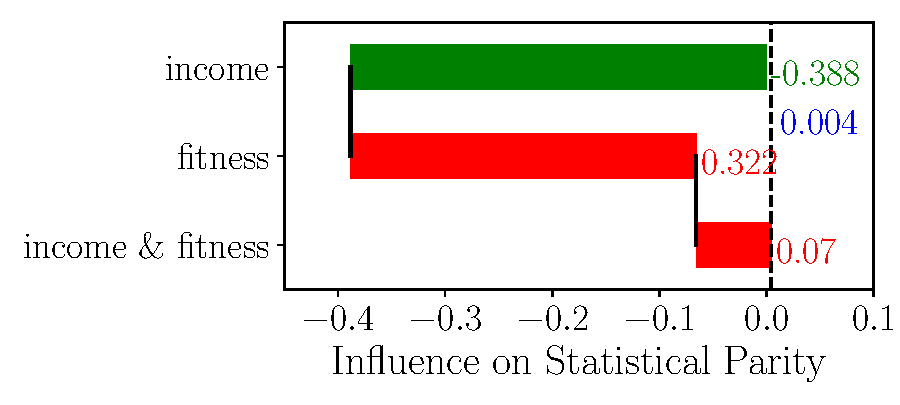
\includegraphics[scale=0.42]{figures/fairness/fif/fif_example_affirmative_action}
		\label{fairness_fairXplainer_fig:fif_affirmative}}
	\end{minipage}
%\vspace*{-.5em}
	\caption[Demonstration of FIF  in health insurance]{FIFs of input features to investigate the bias (statistical parity) of a decision tree predicting the eligibility for health insurance using age-dependent features `fitness' and `income'. An affirmative action reduces bias as corresponding FIFs reflect it.}
	\label{fairness_fairXplainer_fig:fair_example_fif}
	%\vspace{-1.2em}
\end{figure}

We illustrate the usefulness of our contributions via an example scenario proposed in Example~\ref{fairness_justicia_example:intro}. 


%\dbcomment{In recent times, we have observed growing interest to explain sources of unfairness in ML algorithms. Specifically, [a,b] tried to transfer the existing tools from interpretability literature to quantify and explain fairness. But these works mostly demonstrate empirical evaluations to justify the choices of interpretability tools and does not consider the global nature of fairness metrics. In this paper, we develop a formal framework to explain sources of unfairness in an ML algorithm and also a novel methodology to address it. To the best of our knowledge, this is the first work to do so.}


 %\red{This allows practitioners to deploy various affirmative or punitive actions.}\improvement{Examples?}
\begin{example}
	\label{fairness_fairXplainer_ex:motivating_example} We consider a classifier that decides an individual's eligibility for health insurance based on non-sensitive features: fitness  and income. Fitness and income depend on a sensitive feature age $ \in $ \{young, elderly\} leading to two sensitive groups, as highlighted in (Figure~\ref{fairness_fairXplainer_fig:dag_age_income_fitness}--\ref{fairness_fairXplainer_fig:distribution_example}). 
	
	\textbf{Case study 1:} For each sensitive group, we generate $ 1000 $ samples of (income, fitness) and train a decision tree (DT$ 1 $), which predicts without explicitly using the sensitive feature (Figure~\ref{fairness_fairXplainer_fig:dt_original}). %This classifier predicts the eligibility for health insurance without any direct effect of the sensitive feature: age. 	
	Using the $1000$ samples and corresponding predictions, we estimate the statistical parity of DT1 as $ \Pr[\widehat{Y} = 1  \mid  \text{age = young} ] - \Pr[\widehat{Y} = 1  \mid  \text{age = elderly}] = 0.695 - 0.165 = 0.53 $. Therefore, DT$ 1 $ is unfair towards the elderly group.
	
	
	Using the methods described in this chapter, we examine the sources of unfairness in DT$ 1 $ by calculating the FIFs of each feature subset. Positive values represent a reduction in fairness due to increased statistical parity, while negative values indicate an improvement in fairness. The results, shown in the waterfall diagram in Figure~\ref{fairness_fairXplainer_fig:fif_original}, indicate that fitness $(\mathrm{FIF} = 0.355)$, income $(\mathrm{FIF} = 0.098)$, and the combination of income and fitness $(\mathrm{FIF} = 0.055)$ contribute to higher statistical parity and bias. Fitness, being the root of DT$ 1 $, has a greater impact on statistical parity than income, which is at the second level of DT$ 1 $. Our method also reveals the joint effect of income and fitness on statistical parity, which prior methods do not account for (Section~\ref{fairness_fairXplainer_sec:related_work}). The total of the FIFs of all features, $ 0.355 + 0.098 + 0.055 = 0.507 \approx 0.53 $, approximately matches the statistical parity of the classifier, providing a way to break down the bias among all feature subsets. Note that we discuss the estimation error of FIFs in Section~\ref{fairness_fairXplainer_sec:fairxplainer}.
	
%	Now, applying the techniques developed in this paper, we investigate the sources of unfairness of DT$ 1 $ by computing FIFs of features, where \emph{positive numbers indicate reduction in fairness by increasing statistical parity, while negative numbers indicate improvement in fairness}. In the waterfall diagram in Figure~\ref{fairness_fairXplainer_fig:fif_original}, fitness $(\mathrm{FIF} = 0.35)$, income $(\mathrm{FIF}  = 0.1)$, and the joint effect of income and fitness $(\mathrm{FIF}  = 0.05)$ cause higher statistical parity, i.e. higher bias. Intuitively, fitness being at the root of DT$ 1 $ is more influential on statistical parity than income, which is situated at the second level of DT$ 1 $. Our method also reveals the joint (or intersectional) effect of income and fitness on statistical parity, which prior approaches do not consider (Section~\ref{fairness_fairXplainer_sec:related_work}).  Finally, the sum of FIFs of features, $ 0.35 + 0.1 + 0.05 = 0.5 \approx 0.53 $, approximates\footnote{\red{We elaborate on the estimation error of FIFs in Section~\ref{fairness_fairXplainer_sec:fairxplainer}.}} the statistical parity of the classifier, thereby demonstrating a way to decompose the bias of the classifier among all the subsets of features.
	
	
%	\clearpage
	\textbf{Case study 2:} 	
	To address the unfairness of DT$ 1 $ towards the elderly, we introduce DT$ 2 $ which applies an affirmative action. Specifically, for lower fitness, which is typical for the elderly group (Figure~\ref{fairness_fairXplainer_fig:distribution_example}), we decrease the threshold on income from $ 0.69 $ to $ 0.55 $ ({\color{affirmative}green} node in Figure~\ref{fairness_fairXplainer_fig:dt_affirmative}). This allows more elderly individuals to receive insurance as they tend to have higher income, and the lower threshold accommodates their eligibility. The statistical parity of DT$ 2 $ is calculated to be $ \Pr[\widehat{Y} = 1 \mid \text{age = young}] - \Pr[\widehat{Y} = 1 \mid \text{age = elderly}] = 0.707 - 0.706 = 0.001 $, which is negligible compared to the earlier statistical parity of $ 0.53 $ in DT$ 1 $. We estimate the FIFs of features, with $ - 0.388 $ for income, $ 0.322 $ for fitness, and $ 0.07 $ for both features combined. Hence, the negative influence of income confirms the affirmative action, and nullifies the disparity induced by fitness. Additionally, the sum of FIFs $ - 0.388 + 0.322 + 0.07 = 0.004 $ coincides with the statistical parity of DT$ 2 $. 
	
%	Since DT$ 1 $ is unfair to the elderly, we learn another decision tree (DT$ 2 $) by applying an affirmative action. Specifically, for lower fitness, which is typical for the elderly group (Figure~\ref{fairness_fairXplainer_fig:distribution_example}), we decrease the threshold on income from $ 0.69 $ to $ 0.55 $ ({\color{affirmative}green} node in Figure~\ref{fairness_fairXplainer_fig:dt_affirmative}). As {\color{red}the elderly have higher income and} the threshold on income becomes lower for the elderly group, the affirmative action allows more elderly individuals to receive insurance.  Thus, the statistical parity becomes $ \Pr[\widehat{Y} = 1  \mid  \text{age = young}] - \Pr[\widehat{Y} = 1  \mid  \text{age = elderly}] = 0.71 - 0.71 = 0 $, which is negligible than the earlier statistical parity of $ 0.53 $.	Next, we estimate FIFs of features, which are $ - 0.39 $ for income,  $ 0.32 $ for fitness, and $ 0.07 $ for income and fitness together. Hence, the negative influence of income confirms the affirmative action, and nullifies the disparity induced by fitness. We also observe that the sum of FIFs $ - 0.39 + 0.32 + 0.07 = 0 $ coincides with the statistical parity of DT$ 2 $. 
\end{example}



\section{Related Work}
\label{fairness_fairXplainer_sec:related_work}
Recently, local explanation methods have been applied to black-box classifiers to explain sources of bias through feature-attribution\cite{begley2020explainability,lundberg2020explaining} and causal path decomposition\cite{pan2021explaining}. Our work uses the feature-attribution approach and highlights three limitations of existing methods: (i) a failure to estimate intersectional FIFs, (ii) inaccuracies in approximating bias based on FIFs, and (ii) less correlation of FIFs to fairness intervention. Elaborately, to explain group fairness\textemdash a global property of a classifier\textemdash existing local explanation approaches such as ~\cite{begley2020explainability,lundberg2020explaining} estimate FIFs based on a local black-box explainer SHAP~\cite{lundberg2017unified}. They apply a global aggregation (i.e. expectation) of all local explanations corresponding to all data points in a dataset. Such a global aggregation of local explanations is often empirically justified and does not approximate bias accurately (Section~\ref{fairness_fairXplainer_sec:experiments}).  In addition, existing methods ignore the joint contribution of correlated features on bias. To address these limitations, \textit{we develop a formal framework to explain sources of group unfairness in a classifier and also a novel methodology to estimate FIFs. To the best of our knowledge, this is the first work to do both}.


%Recently, several studies apply \emph{local explanation methods} for black-box classifiers to explain sources of bias by feature-attribution~\cite{begley2020explainability,lundberg2020explaining} and causal path decomposition~\cite{pan2021explaining}. Our work adopts feature-attribution approach and reveals two-fold limitations of existing methods: (i) \emph{inaccuracy} in approximating bias in terms of estimated FIFs and (ii) \emph{failing to estimate intersectional} FIFs. Elaborately, to explain group fairness\textemdash a global property of a classifier\textemdash existing local explanation approaches such as ~\cite{begley2020explainability,lundberg2020explaining} estimate FIFs based on a local black-box explainer SHAP~\cite{lundberg2017unified}. They apply a global aggregation (such as expectation) of all local explanations corresponding to all data points in a dataset. Such a global aggregation of local explanations is often empirically justified and does not approximate bias accurately (Section~\ref{fairness_fairXplainer_sec:experiments}). In addition, features are often correlated in practical fairness tasks, and computing only individual FIFs ignores the joint contribution of multiple features on the bias of the classifier. To this end,  in this paper, \textit{we develop a formal framework to explain sources of group unfairness in a classifier and also a novel methodology to address it. To the best of our knowledge, this is the first work to do both}. %\todo{1. GSA with fairness, 2. Citation not correct, 3. Influence of Yair Zick.}

Among other related works, \cite{benesse2021fairness} links GSA measures such as Sobol and Cram{\'e}r-von-Mises indices to different fairness metrics. While their approach relates the GSA of sensitive features on bias, we focus on applying GSA to all features to estimate FIFs. \textit{Their approach detects the presence or absence of bias, while we focus on decomposing bias as the sum of FIFs of all feature subsets}. In another line of work, \cite{datta2016algorithmic} and \cite{ghosh2022algorithmic} estimate feature-influence as the shifting of bias from its original value by randomly intervening features. Their work is different from the decomposability property of FIFs, where the sum of FIFs is equal to the bias. A separate line of work estimates the fairness influence of data points in a dataset~\cite{li2022achieving,wang2022understanding}, while \textit{our focus is on quantifying influences of input features}.
